%%%%%%%%%%%%%%%%%%%%%%%%%%%%%%%%%%%%%%%%%
% baposter Landscape Poster
% LaTeX Template
% Version 1.0 (11/06/13)
%
% baposter Class Created by:
% Brian Amberg (baposter@brian-amberg.de)
%
% This template has been downloaded from:
% http://www.LaTeXTemplates.com
%
% License:
% CC BY-NC-SA 3.0 (http://creativecommons.org/licenses/by-nc-sa/3.0/)
%
%%%%%%%%%%%%%%%%%%%%%%%%%%%%%%%%%%%%%%%%%

%----------------------------------------------------------------------------------------
%	PACKAGES AND OTHER DOCUMENT CONFIGURATIONS
%----------------------------------------------------------------------------------------

\documentclass[landscape,a0paper,fontscale=0.285]{baposter} % Adjust the font scale/size here

\usepackage{graphicx} % Required for including images
\graphicspath{{figures/}} % Directory in which figures are stored

\usepackage{amsmath} % For typesetting math
\usepackage{amssymb} % Adds new symbols to be used in math mode

\usepackage{booktabs} % Top and bottom rules for tables
\usepackage{enumitem} % Used to reduce itemize/enumerate spacing
\usepackage{palatino} % Use the Palatino font
\usepackage[font=small,labelfont=bf]{caption} % Required for specifying captions to tables and figures

\usepackage{multicol} % Required for multiple columns
\setlength{\columnsep}{1.5em} % Slightly increase the space between columns
\setlength{\columnseprule}{0mm} % No horizontal rule between columns

\usepackage{tikz} % Required for flow chart
\usetikzlibrary{shapes,arrows} % Tikz libraries required for the flow chart in the template

\newcommand{\compresslist}{ % Define a command to reduce spacing within itemize/enumerate environments, this is used right after \begin{itemize} or \begin{enumerate}
\setlength{\itemsep}{1pt}
\setlength{\parskip}{0pt}
\setlength{\parsep}{0pt}
}

\definecolor{lightblue}{rgb}{0.145,0.6666,1} % Defines the color used for content box headers

\begin{document}

\begin{poster}
{
headerborder=closed, % Adds a border around the header of content boxes
colspacing=1em, % Column spacing
bgColorOne=white, % Background color for the gradient on the left side of the poster
bgColorTwo=white, % Background color for the gradient on the right side of the poster
borderColor=lightblue, % Border color
headerColorOne=black, % Background color for the header in the content boxes (left side)
headerColorTwo=lightblue, % Background color for the header in the content boxes (right side)
headerFontColor=white, % Text color for the header text in the content boxes
boxColorOne=white, % Background color of the content boxes
textborder=roundedleft, % Format of the border around content boxes, can be: none, bars, coils, triangles, rectangle, rounded, roundedsmall, roundedright or faded
eyecatcher=true, % Set to false for ignoring the left logo in the title and move the title left
headerheight=0.1\textheight, % Height of the header
headershape=roundedright, % Specify the rounded corner in the content box headers, can be: rectangle, small-rounded, roundedright, roundedleft or rounded
headerfont=\Large\bf\textsc, % Large, bold and sans serif font in the headers of content boxes
%textfont={\setlength{\parindent}{1.5em}}, % Uncomment for paragraph indentation
linewidth=2pt % Width of the border lines around content boxes
}
%----------------------------------------------------------------------------------------
%	TITLE SECTION 
%----------------------------------------------------------------------------------------
%
{
\includegraphics[height=6em]{duke_univ_blue.png}} % First university/lab logo on the left
{\bf\textsc{Distinguish Malignant From Benign Breast Cancer}\vspace{0.5em}} % Poster title
{\textsc{Xin Liu, Jingzhu Zhou and Mengshu Shao  \hspace{12pt} Department of Biostatistics \& Bioinformatics}} % Author names and institution
% Second university/lab logo on the right
{
\includegraphics[height=7em]{biostat_logo.jpeg}} 
%----------------------------------------------------------------------------------------
%	OBJECTIVES
%----------------------------------------------------------------------------------------

\headerbox{Introduction and Objectives}{name=objectives,column=0,row=0,span=2}{

\begin{multicols}{2}
Objective:The goal of this work is to use machine learning methodology to develop digitalized method to minimize subjectivity of the visual diagnosis and increase accuracy of classification for each breast cancer patient.

Introduction: Breast cancer stage can be diagnosed by visually examining fine needle aspirate cancer cell images. The accuracy of the diagnosis is over 90\%.  However, there exists large standard error for the mean sensitivity and the mean specificity of the diagnosis. This indicates the accuracy varies greatly within individual series and visual diagnosis involves a great deal of subjectivity. 
\end{multicols}
}


\vspace{0.3em} % When there are two boxes, some whitespace may need to be added if the one on the right has more content


%----------------------------------------------------------------------------------------
%	INTRODUCTION
%----------------------------------------------------------------------------------------


%----------------------------------------------------------------------------------------
%	RESULTS 1
%----------------------------------------------------------------------------------------

\headerbox{Results 2}{name=results,column=2,span=2,row=0}{

\begin{multicols}{2}
\vspace{1em}
{\bf{1. Ridge parameter selection}}
\begin{center}
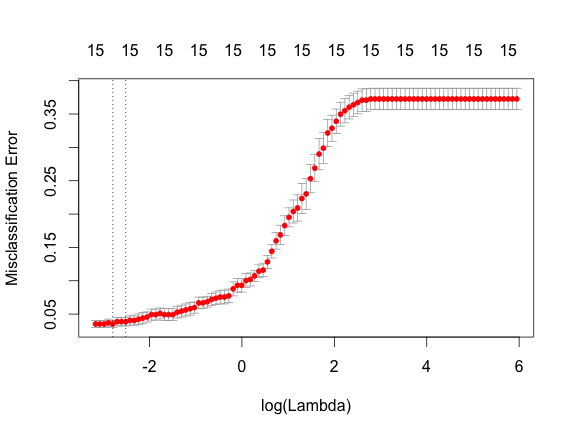
\includegraphics[width=0.7\linewidth]{Rplot}


\end{center}

 The best tuning parameter:0.00304. Then Ridge regression was used to fit the model based on the tuning parameter. 

\begin{center}
$logit(P(Y_i=1|X=x))= -9.35+0.073texture_m+4.74concavity_m+14.72concave_points_m-39.34fractal_m+1.81radius_sd-0.13texture_sd-8.03smoothness_sd-2.52compactness_sd-56.07fractal_sd+0.15radius_w +0.06texture_w+12.44smoothness_w +1.58concavity_w+8.59concave_points_w+4.41symmetry_w$
\end{center} 


\end{multicols}

%------------------------------------------------


\vspace{1em}
{\bf{2.Varying SVM input parameters }}\\
In another set of experiments we studied the dependence of the training error found by the SVM algorithm on the parameter C. Table 2 shows the variation of the training error corresponds with the parameter C. It can be seen that the smallest error is obtained for C=0.9.


\begin{center}
\begin{tabular}{l l l l l l l l l l l} 
\toprule
\textbf{Cost} & \textbf{0.1} & \textbf{0.2} & \textbf{0.3} & \textbf{0.4} & \textbf{0.5} & \textbf{0.6} & \textbf{0.7} & \textbf{0.8} & \textbf{0.9} & \textbf{1.0}\\
\midrule
\textbf{Accuracy} & 93.85 & 95.08 & 96.31 & 96.49 & 96.84 & 97.19 & 97.19 & 97.54 & 97.72 & 97.36 \\
\bottomrule
\end{tabular}
\captionof{table}{Parameter selection for SVM}

\end{center}


}

%----------------------------------------------------------------------------------------
%	REFERENCES
%----------------------------------------------------------------------------------------

\headerbox{References}{name=references,column=0,span=3,above=bottom}{


\begin{multicols}{3}
\renewcommand{\section}[2]{\vskip 0.05em} % Get rid of the default "References" section title
\nocite{*} % Insert publications even if they are not cited in the poster
\small{ % Reduce the font size in this block
\bibliographystyle{unsrt}
\bibliography{10.1111_j.1524-4741.1997.tb00145.x,scholar,science} % Use sample.bib as the bibliography file

}

\end{multicols}
}

%----------------------------------------------------------------------------------------
%	FUTURE RESEARCH
%----------------------------------------------------------------------------------------


%----------------------------------------------------------------------------------------
%	CONTACT INFORMATION
%----------------------------------------------------------------------------------------

\headerbox{Contact Information}{name=contact,column=3,aligned=references,above=bottom}{ % This block is as tall as the references block

\begin{description}\compresslist
\item[Email] xin.liu1@duke.edu
\item            mengshu.shao@duke.edu
\item            jingzhu.zhou@duke.edu
\end{description}
}

%----------------------------------------------------------------------------------------
%	CONCLUSION
%----------------------------------------------------------------------------------------

\headerbox{Conclusion}{name=conclusion,column=2,span=2 ,below=results,above=references}{

\begin{center}
\begin{tabular}{l l l l l l} 
\toprule
\textbf{Model} & \textbf{Logistic} & \textbf{Ridge} & \textbf{LDA} & \textbf{QDA} & \textbf{SVM}\\
\midrule
Accuracy & 96.14 & 96.49 & 95.96 & 94.91 & 97.72\\
Predictor numbers & 8 & 15 & 8 & 8 &24 \\
\bottomrule
\end{tabular}
\captionof{table}{Model Comparison}

\end{center}





%------------------------------------------------

\begin{itemize}\compresslist
\item All models give an accuracy rate above 95 \%. Support vector machines gave the best accuracy, however it used the highest number of parameters. 
\item We would recommend logistic regression since it gave comparably high accuracy with the lowest number of parameters. 
\item Future Research:The various fitted models can be tested for accuracy, sensitivity and specificity on testing data (future patients prognosis) based on those cell measurements.Other classification methods such as extended bases LDA, QDA, plus interaction terms could be considered.

\end{itemize}





}



%----------------------------------------------------------------------------------------
%	MATERIALS AND METHODS
%----------------------------------------------------------------------------------------

\headerbox{Materials \& Methods}{name=method,column=0,below=objectives,bottomaligned=conclusion}{ % This block's bottom aligns with the bottom of the conclusion block

The following classification methods were considered in this research:

\begin{itemize}\compresslist
\item Logistic regression
\item Penalized logistic regression (LASSO plus Ridge)
\item Linear / Qudratic Discriminant Analysis
\item Support Vector Machine
\end{itemize}

The dataset contains records of 569 breast cancer instances, in which:
\begin{multicols}{2}
\begin{itemize}
\item 212 malignant
\item 357 benign
\end{itemize}
\end{multicols}
Thirty variables are computed for each cell nucleus for breast cancer diagnosis prediction including mean(\_m), sd(\_sd), mean of largest three(\_w) for the following features: 
\begin{multicols}{2}
\begin{description}\compresslist
\item 1) radius              
\item 2) texture
\item 3) perimeter         
\item 4) area  
\item 5) smoothness
\item 6) compactness
\item 7) concavity
\item 8) concave points
\item 9) symmetry
\item 10) fractal dimension             
\end{description}
\end{multicols}


\tikzstyle{decision} = [diamond, draw, fill=blue!20, text width=4.5em, text badly centered, node distance=2cm, inner sep=0pt]
\tikzstyle{block} = [rectangle, draw, fill=blue!20, text width=6em, text centered, rounded corners, minimum height=4em]
\tikzstyle{line} = [draw, -latex']
\tikzstyle{cloud} = [draw, ellipse, fill=red!20, node distance=3cm, minimum height=2em]



\begin{tikzpicture}[node distance = 2.7cm, auto]
\node [block] (init) {Model Selection};

\node [block, right of=init] (init2) {Classification};
\node [block, right of=init2] (End) {Model Comparsion};
\path [line] (init) -- (init2);
\path [line] (init2) -- (End);

\end{tikzpicture}



}

%----------------------------------------------------------------------------------------
%	RESULTS 2
%----------------------------------------------------------------------------------------

\headerbox{Results 1}{name=results2,column=1,below=objectives,bottomaligned=conclusion}{ % This block's bottom aligns with the bottom of the conclusion block


Model Selection for LDA,QDA,SVM:
\begin{itemize}
\item 1.Pairwise correlations of the 30 variables were used to delete the variables that are highly correlated. Variable deleted: radius\_m,perimeter\_m,area\_w,perimeter\_w,
radius\_w,area\_sd,perimeter\_sd
\item 2.Stepwise selection(logistic regression) were used to select the best subset of variables based on lowest AIC. Variable selected: concave\_points\_w, area\_m, texture\_w,radius\_sd,compactness\_sd,
smoothness\_w,concavity\_w ,texture\_sd
\end{itemize}

Model Selection for Penalized Regression:
\begin{itemize}
\item
Lasso uses the constraint of the overall magnitude of the coefficients, thus important predictors are included in the model, and less important predictors shrink, potentially to zero. 10-folds cross validation selects the tuning parameter which makes the smallest cross validation error. 
\item
The variables selected are texture\_m, concavity\_m, concave\_points\_m, fractal\_m, radius\_sd, texture\_sd, smoothness\_sd, compactness\_sd, fractal\_sd, radius\_w, texture\_w, smoothness\_w, concavity\_w, concave\_points\_w and symmetry\_w.

\end{itemize}


}

%----------------------------------------------------------------------------------------

\end{poster}

\end{document}